	\section{Прикладные задачи}
	\subsection{Многоагентная постановка}
	\begin{frame}
		\frametitle{Особенности постановки задачи}
		
		Рассматривается случай группового взаимодействия автономных технических объектов (агентов), в котором:
		\begin{itemize}
			\item агенты решают общую задачу (имеют общую цель высшего уровня),
			\item агенты действуют независимо друг от друга (децентрализованное управление), в т.ч. могут ставить индивидуальные подцели и достигать их,
			\item агенты обладают различными характеристиками, как техническими, так и когнитивными, т.е. разными стратегиями поведения,
			\item агенты обладают различными картинами мира,
			\item агенты действуют в меняющейся среде.
		\end{itemize}
		
	\end{frame}
	
	\begin{frame}
		\frametitle{Требования к представлению знаний}
		
		На представление пространственных и временных знаний в задаче согласованного перемещения с такими особенностями налагается ряд ограничений:
		\begin{itemize}
			\item необходимость поддержки некоторого протокола коммуникации, разделение знаний на коммуницируемые и некоммуницируемые (личные),
			\item необходимость выделения компоненты знания, не зависящей от индивидуальных (личных) характеристик агента,
			\item требование к наличию механизма связывания реальных объектов внешней среды и процедур их распознавания с символьным коммуницируемым представлением (symbol grounding problem),
			\item поддержка механизмов пополнения картины мира (обучение и абстрагирование).
		\end{itemize}
	\end{frame}

	\begin{frame}
		\frametitle{Практические задачи}
		
		\centering
		\includegraphics[width=\textwidth]{examples/signs/robotic_signs}

	\end{frame}
	
	\subsection{Задача интеллектуального перемещения}
	\begin{frame}
		\frametitle{Задача интеллектуального перемещения}
		
		\begin{columns}
			\begin{column}{0.55\textwidth}
				\begin{center}
					\includegraphics[page=1,width=0.8\textwidth]{examples/plan/slides_colored}
				\end{center}
				\vspace{-7pt}
				\small
				\textbf{Задача}
				
				Целевая область не достижима некоторым агентом самостоятельно (с использованием только методов планирования траектории).
				
				\textbf{Решение}
				
				Агенты должны поддерживать коммуникацию и модифицировать свои собственные планы с учетом коалиционных подзадач.
				
			\end{column}
			\begin{column}{0.45\textwidth}
				Особенности:
				\begin{itemize}
					\item Меняющаяся внешняя среда.
					\item Различные типы препятствий (некоторые могут быть разрушены).
					\item Агенты обладают различной функциональностью.
					\item Общая пространственная цель (ВСЕ агенты должны достичь определенной области на карте).
				\end{itemize}
			\end{column}
		\end{columns}
	\end{frame}
	
	\begin{frame}
		\frametitle{Распределение ролей при решении задачи}
		\begin{center}
			\scalebox{0.7}{
				\animategraphics{12}{examples/plan/slides_colored}{}{}			
			}
		\end{center}
	\end{frame}


	\begin{frame}
		\frametitle{Представление пространственных знаний}
		
		\begin{columns}
			\begin{column}{0.7\textwidth}
				\includegraphics[width=\textwidth]{examples/representations/bica_psy_path.png}
			\end{column}
			\begin{column}{0.3\textwidth}
				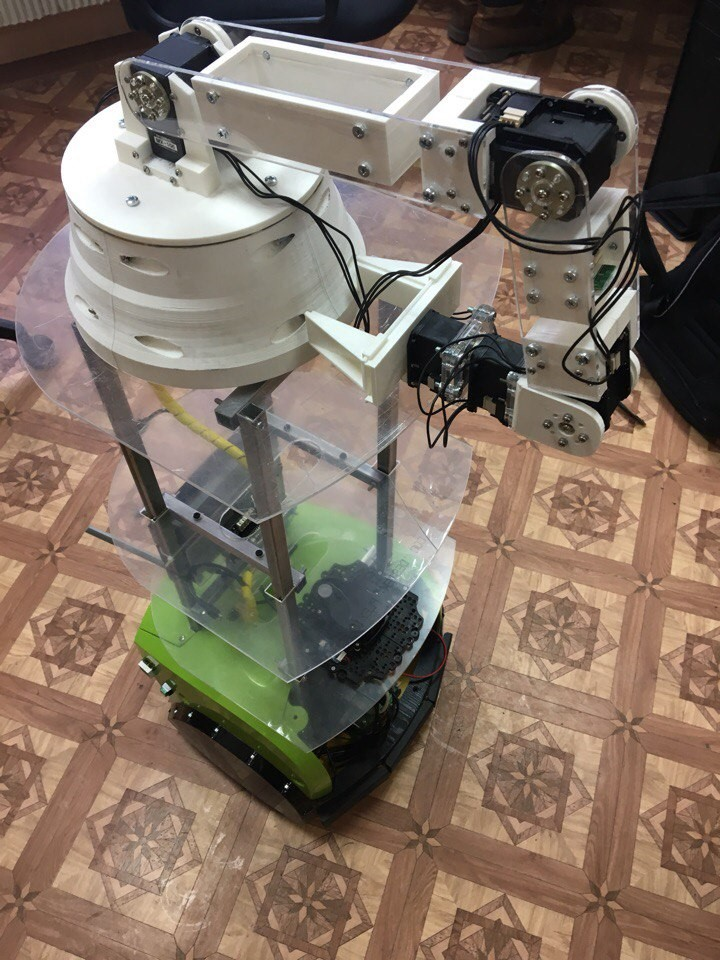
\includegraphics[width=\textwidth]{nexus.jpg}
			\end{column}
		\end{columns}
		
		\nocite{*}
		\printbibliography[keyword={behplanrus}, resetnumbers=true]
	\end{frame}	

	\begin{frame}
		\frametitle{Представление действий по перемещению}
		
		Действия по перемещению "--- знаки $s_t$ (признаки $f_t$, $t$ "--- тип перемещения), которым соответствуют каузальные матрицы типа $Z_t$, состоящие из трёх столбцов 
		\[
		z_1=(l_x, I), z_2=(l_y, d_u, E), z_3=(l_y, I, t_v),
		\]
		где 
		\begin{itemize}
			\item $l_x$, $l_y$ "--- признаки, соответствующие категории расстояния в пространственной логике  (например, вплотную, близко, далеко и др.), 
			\item $d_u$ "--- признак, соответствующий категории направления в пространственной логике (например, впереди, слева и др.), 
			\item $t_v$ "--- признак, соответствующий категории времени во временной логике (например, скоро, в будущем и др.),
			\item $I$ "--- признак присутствия самого агента, 
			\item $E$ "--- признак отсутствия препятствия.
		\end{itemize}
	\end{frame}	
	
	\begin{frame}
		\frametitle{Представление пространственных знаний}
		
		\begin{columns}
			\begin{column}{0.55\textwidth}
				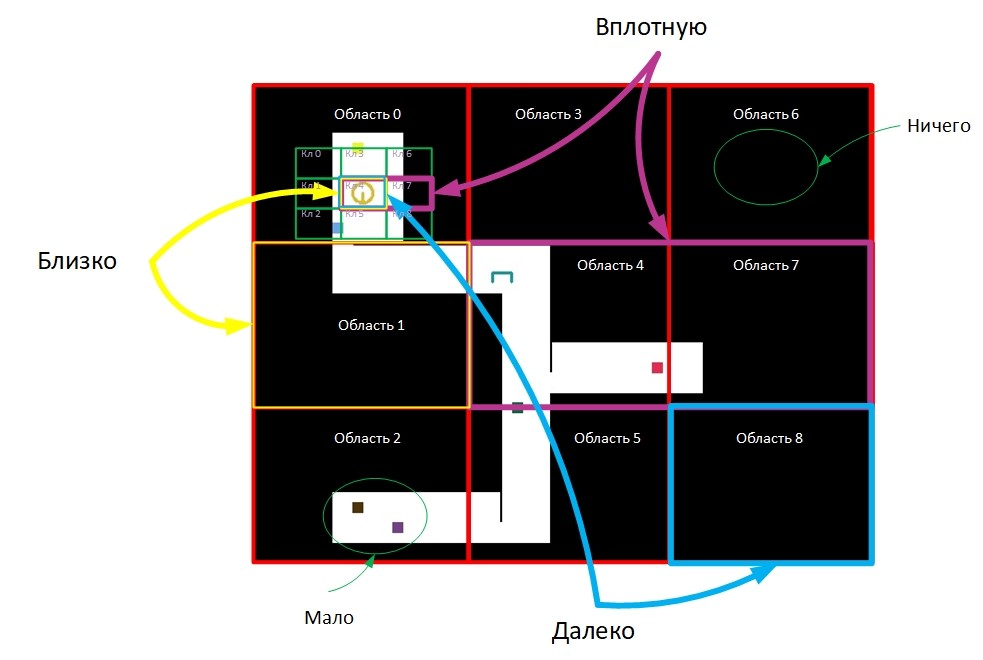
\includegraphics[width=\textwidth]{areas.jpg}
			\end{column}
			\begin{column}{0.45\textwidth}
				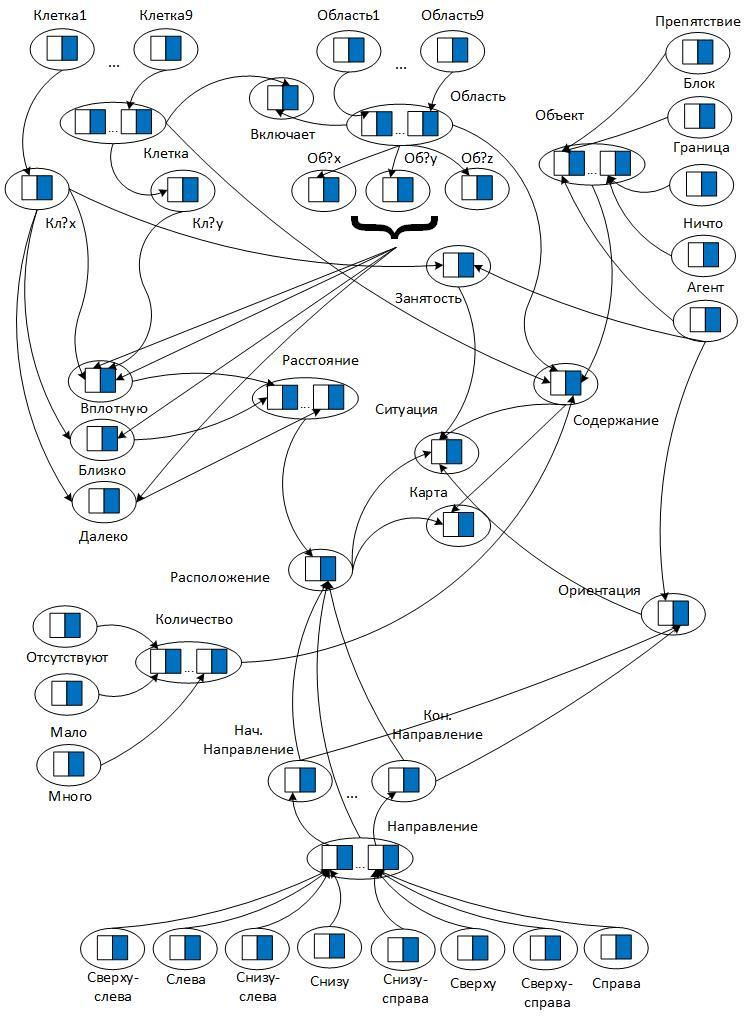
\includegraphics[width=\textwidth]{areas_signif.jpg}
			\end{column}
		\end{columns}
	\end{frame}
	\subsection{Распределение ролей в коллективе}
	\begin{frame}
		\frametitle{Знаки Я и Они в алгоритме планирования MAP}
		
		\begin{center}
			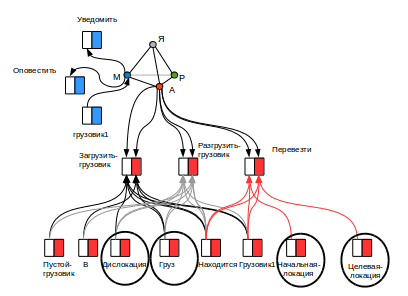
\includegraphics[width=0.6\textwidth]{I-sign.png}
			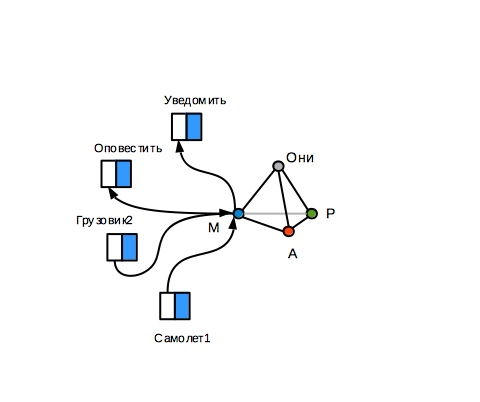
\includegraphics[width=0.5\textwidth]{they-sign.png}
		\end{center}
		\nocite{*}
		\printbibliography[keyword={roledistrib}, resetnumbers=true]
	\end{frame}
	\subsection{Обучение с подкреплением}
	\begin{frame}
		\frametitle{Подкрепление для формирования\\каузальных матриц}
		\footnotesize
		
		\begin{columns}
			\begin{column}{0.5\textwidth}
				\centering
				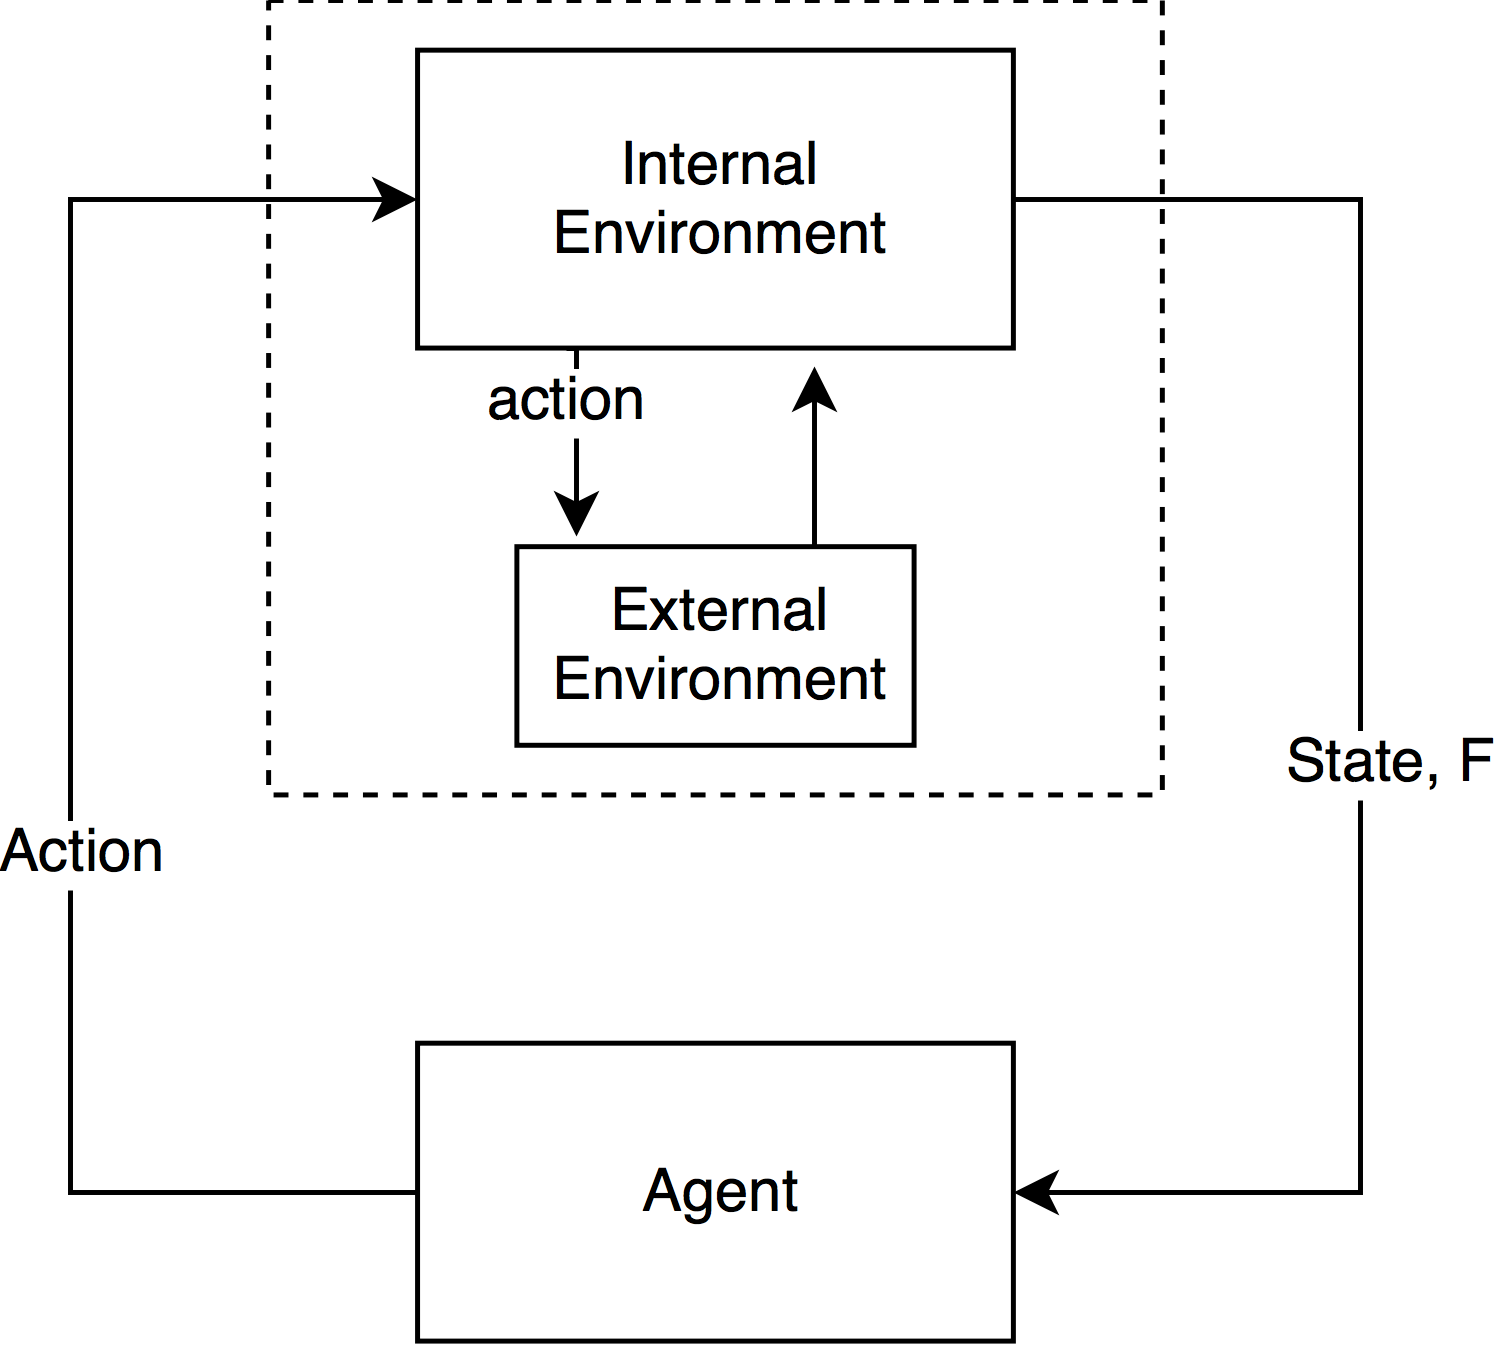
\includegraphics[width=0.7\textwidth]{schema.png}
			\end{column}
			\begin{column}{0.5\textwidth}
				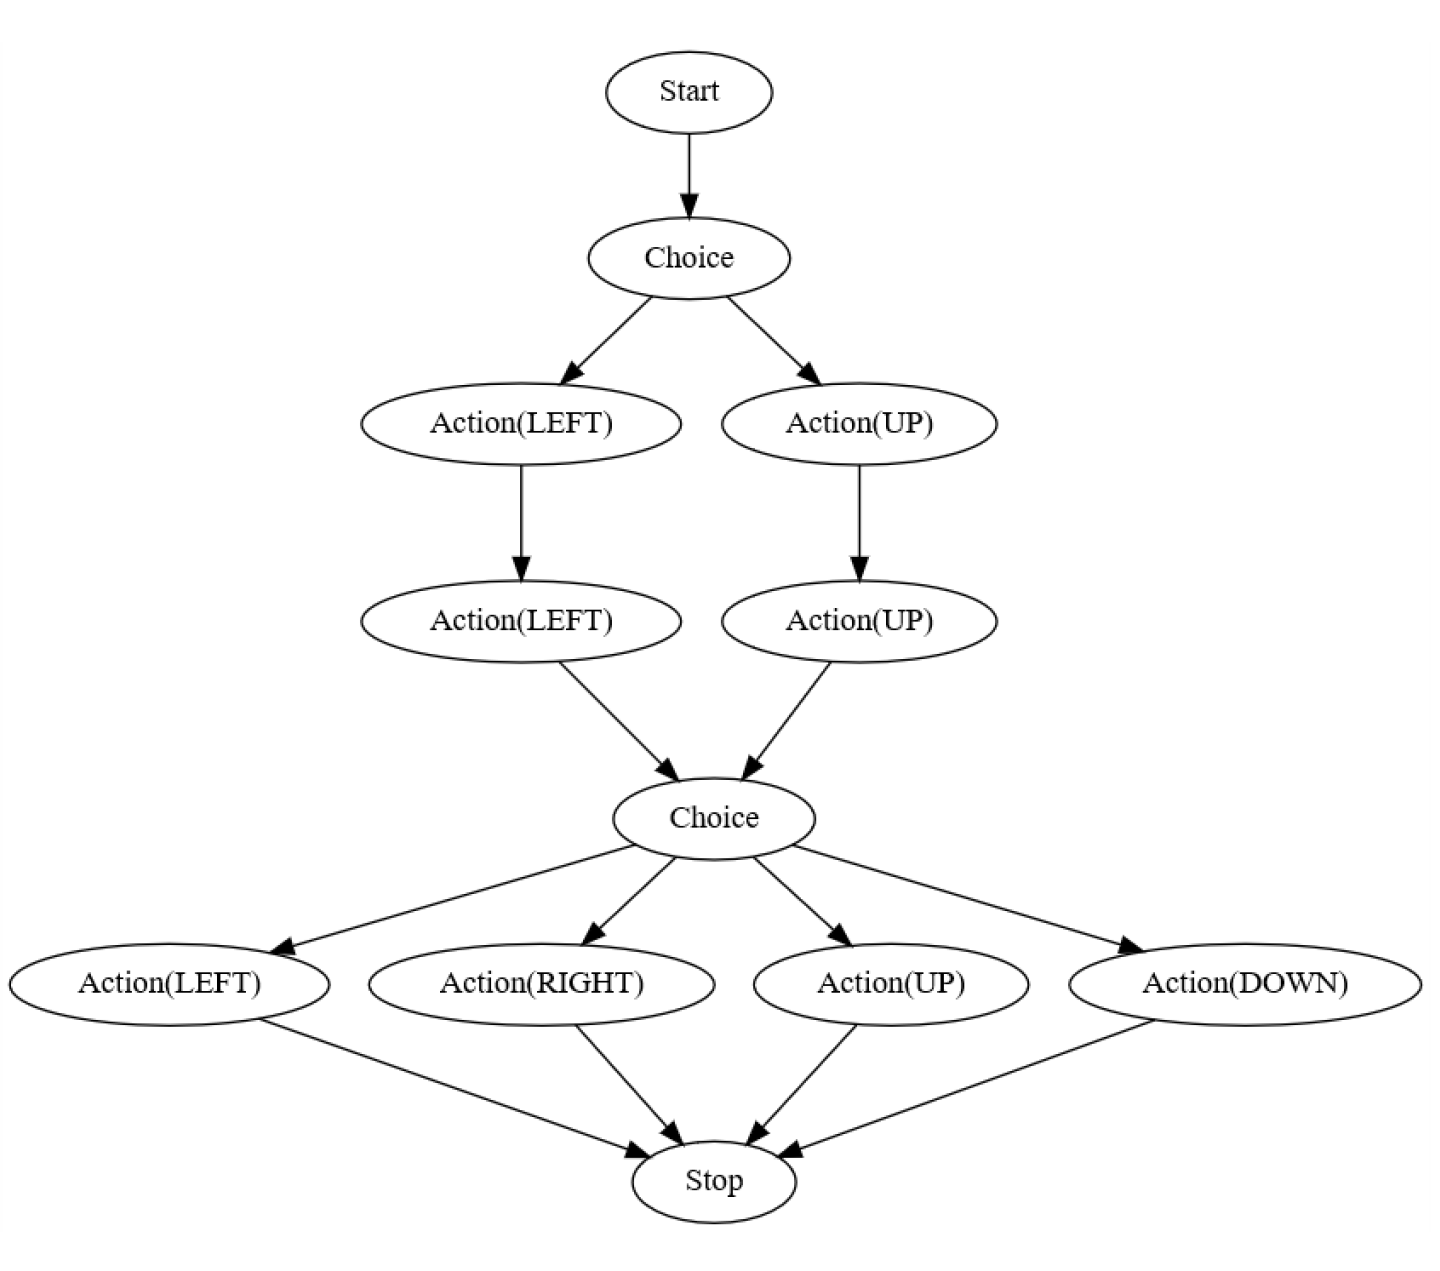
\includegraphics[width=0.8\textwidth]{autoham.png}
			\end{column}
		\end{columns}
		
		
		\begin{itemize}
			\item \textbf{Иерархическое обучение с подкреплением} для формирования представления о новых действиях.
			\item Чередование процессов абстрагирования действий и абстрагирования состояний среды.
			\item Автоматическое формирование иерархии операций.
		\end{itemize}
	
	\end{frame}	